% Capitulo 4

\chapter{Um protótipo de serviço federado}
\label{Capitulo4}
\lhead{Cap\'itulo 4. \emph{Um protótipo de serviço federado}}

O uso de tecnologias digitais oferece novas possibilidades para o
ensino e a formação. Muitas comunidades, aferentes a RM, tem começando
produzir material pedagógico audiovisual, que com a ajuda da rede,
poderia contribuir para enriquecer os programas educacionais públicos,
geralmente deficientes e pouco integrados com a cultura quilombola. O
\emph{Núcleo de Pesquisa e Desenvolvimento Digital (NPDD)}\footnote{O
  \emph{Núcleo de Pesquisa e Desenvolvimento Digital (NPDD)} da RM
  pesquisa e desenvolve tecnologias para a comunicação, a produção de
  energias renováveis e sustentáveis, e a melhoria das condições de
  vida em simbiose com o ambiente. Mais informações em
  \url{http://wiki.mocambos.net/wiki/NPDD}.} da RM, com o projeto
\emph{Tambor e Comunicação}\footnote{O projeto \emph{Tambor e
    Comunicação} tenta fortificar a rede de comunicação digital
  seguindo as necessidades das comunidades. Ver
  \url{http://wiki.mocambos.net/wiki/Projeto_Tambor_e_Comunicacao}.},
propus a pesquisa e o desenvolvimento de uma solução para a publicação
e compartilhamento em rede de imagens, áudios e vídeos de interesse
comum e geralmente produzidos nas comunidades. 

\section{Sistema de publicação e difusão de conteúdos multimídia}
O sistema desenvolvido prevê a instalação de um portal no servidor
local das comunidades através do qual é possível visualizar e publicar
conteúdos multimídia aproveitando a rapidez da rede local. O sistema
cuida de memorizar os conteúdos em um acervo multimídia local e
compartilhar, aqueles etiquetados como de interesse comum, com os
servidores das outras comunidade (ver figura
\ref{fig:SchemaServer_ReteMocambos}). O protótipo tenta resolver as
limitações de banda da conexão respeitando a especificação dos
requisitos.

\begin{figure}[htbp]
  \centering
  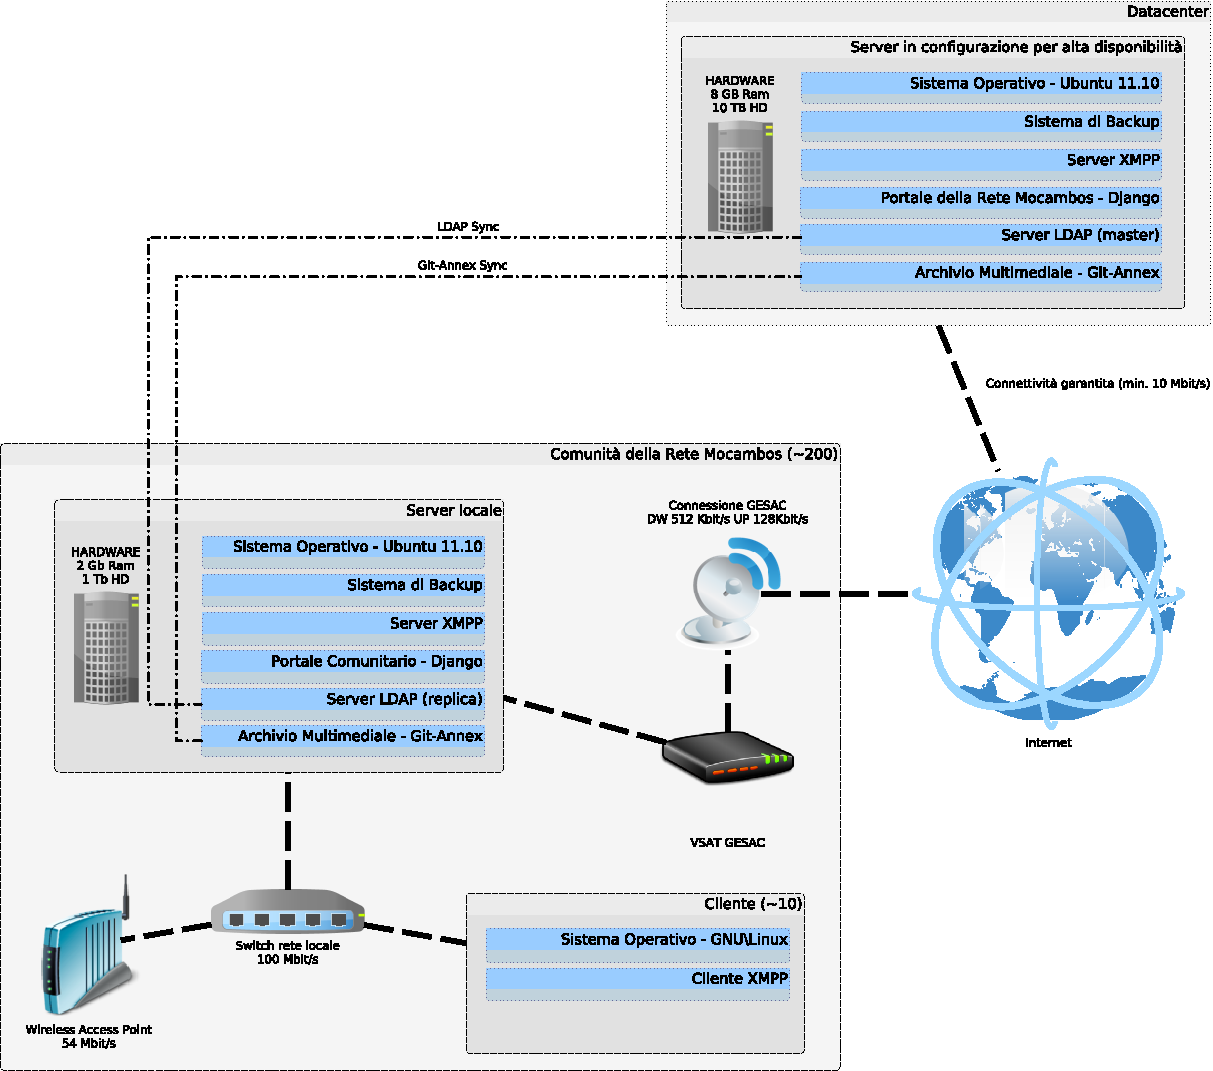
\includegraphics[width=\textwidth]{./Figure/SchemaServer_ReteMocambos-crop.pdf}
  \rule{35em}{0.5pt}
  \caption[Esquema da infraestrutura da RM]{Esquema da infraestrutura da RM.}
  \label{fig:SchemaServer_ReteMocambos}
\end{figure}

\section{Acervo multimídia}
O acervo multimídia local da comunidade é um repositório
\emph{git-annex} (ver \ref{git-annex}) que vem gerenciado através de
um portal comunitário, seja pela publicação seja pela visualização dos
conteúdos. O acesso direto aos dados é todavia garantido sendo esses
arquivos acessíveis no disco. Também é possível interagir com os dados
através do amplo universo de aplicações e bibliotecas do
\emph{git}. Em especial o protótipo usa a estrutura de metadados do
\emph{git} para manter o controle do usuário que publicou um
conteúdo. A operação de \emph{commit} coincide da facto com a
publicação de um conteúdo, e o \emph{committer} com o usuário que o
publica. Os metadados, em vez, relativos ao conteúdo multimídia em si,
como autor, tipo de licenciamento, data de criação, podem ser
memorizados internamente ao arquivo seguindo os padrões existentes
como o \emph{Dublin Core}\footnote{``O Dublin Core é um sistema de
  metadados que contempla um núcleo de elementos essenciais para a
  descrição de qualquer conteúdo digital acessível via rede.'',
  traduzido de Wikipedia:
  \url{http://it.wikipedia.org/wiki/Dublin_Core}.}.

Um elemento importante para o acervo multimídia são as operações de
sincronização. As ferramentas baseadas no \emph{git} herdam a sua
natureza descentralizada e a capacidade de comunicar de forma
transparente usando vários protocolos. Em particular é interessante a
possibilidade de executar sincronizações com sistemas de armazenamento
massivo, característica essencial na fase de criação de um novo nó,
onde a primeira sincronização via rede poderia levar dias (ver
requisito \ref{Sincronizzazione}). As transferências contudo, no caso
do \emph{git-annex}, são executadas através do protocolo
\emph{rsync}\footnote{\emph{rsync} é um Software Livre para a
  transfêrencia rápida e incremental de arquivos disponível no
  \url{http://rsync.samba.org/}.}, que gerencia eventuais
interrupções, evitando retransmissões onerosas. 

\subsection{git-annex}\label{git-annex}
\emph{git-annex}\footnote{\emph{git-annex} é um proframa que estende
  as funcionalidades do \emph{git} em gerir arquivos de grande tamanho
disponível no \url{http://git-annex.branchable.com}.} permite a
gestão de arquivos com \emph{git}, sem a necessidade de adicionar os
arquivos dentro \emph{git}. Mesmo se pode parecer paradoxal, é útil
quando se trabalha com arquivos muito grandes que \emph{git}
atualmente não gerencia facilmente por limitações devidas a memoria,
tempo ou espaço no disco.

Mesmo sem manter o histórico das mudanças do conteúdo do arquivo, ter
a possibilidade de gerenciar arquivos com \emph{git}, de movê-los, e
exclui-los, numa arvore de pasta versionada, com uso de
\emph{branches} e de clones distribuídos, são todos bons motivos para
usar \emph{git}. E os arquivos anexos (por isso o nome
\emph{git-annex}) podem coexistir no mesmo repositório \emph{git} com
os arquivos regularmente versionados. 

\emph{git-annex} transforma os arquivos anexos em \emph{link}
simbólicos, que são normalmente versionados por \emph{git}. 

O conteúdo dos arquivos é mantido por \emph{git-annex} em um acervo
chave/valor distribuído que corresponde aos clones de um dado
repositório \emph{git}. Praticamente \emph{git-annex} memoriza o
conteúdo do arquivo em uma subpasta de \verb|.git/annex/|.

A primeira vez que um arquivo é adicionado no \emph{git-annex}, é
calculada uma chave, normalmente fazendo um \emph{hash} do seu
conteúdo. \emph{git-annex} todavia suporta vários \emph{backend} que
podem produzir diferentes tipos de chaves. O arquivo que é adicionado
no \emph{git} nada mais é que um \emph{link} simbólico para a chave
memorizada no \verb|.git/annex/|. Se o conteúdo do arquivo for
modificado, é gerada uma outra chave, e o \emph{link} é alterado. 

O conteúdo do arquivo pode ser transferido de um repositório para
outro por \emph{git-annex}, que além de manter controle de quem mantem
o que, permite criar um mapa das copias disponíveis e impor um numero
minimo de copias. Essas informações são mantidas em um \emph{branch}
separado, chamado ``\emph{git-annex}'', e as operações de
sincronização, são simplesmente \emph{push} e \emph{pull} entre os
vários clones dos repositórios.

\emph{git-annex} suporta:
\begin{itemize}
\item localização das copias (\emph{location tracking})
\item download seletivo dos conteúdos 
\item gestão da confiança dos repositórios
\item gestão do numero minimo de copias
\item vários \emph{backend} para as chaves (SHA\footnote{Secure Hash
    Algoritm, (SHA), é um algoritmo usado em sistemas chave/valor onde
    as chaves são calculadas através de uma função criptográfica dos
    valores.}, WORM\footnote{O algoritmo WORM identifica os arquivos
    em base ao nome, dimensão e data de alteração.})
\item vários \emph{backend} para os conteúdos/valores
  (BUP\footnote{BUP é um sistema para \emph{backup} a alta eficiência
    disponível no: \url{https://github.com/apenwarr/bup}.}, rsync,
  web, S3\footnote{Amazon Simple Storage Service, (S3) é uma
    infraestrutura para a memorização dos dados totalmente redundante,
    disponível no: \url{aws.amazon.com/}.})
\end{itemize}

\section{Portal Comunitário}
O portal local tem que oferecer acesso aos principais serviços locais
da comunidade. Para o desenvolvimento foi escolhido o uso de um
framework baseado no Python, \emph{Django} (ver \ref{Django}), que
possibilita uma integração flexível e avançada com outros sistemas
graças as numerosas bibliotecas disponíveis como, por exemplo, para a
autenticação LDAP.

Para a instalação do framework e do modelo de base do protótipo de
portal comunitário foi criado um \emph{script} enquanto, para gerir o
acervo multimídia \emph{git-annex} foram desenvolvidos duas aplicações
para \emph{Django}, que definem o modelo dos dados e cuidam de
adicionar os conteúdos no repositório executando as operações de
\emph{commit}, \emph{push} e \emph{pull}.

\begin{figure}[htbp]
  \centering
  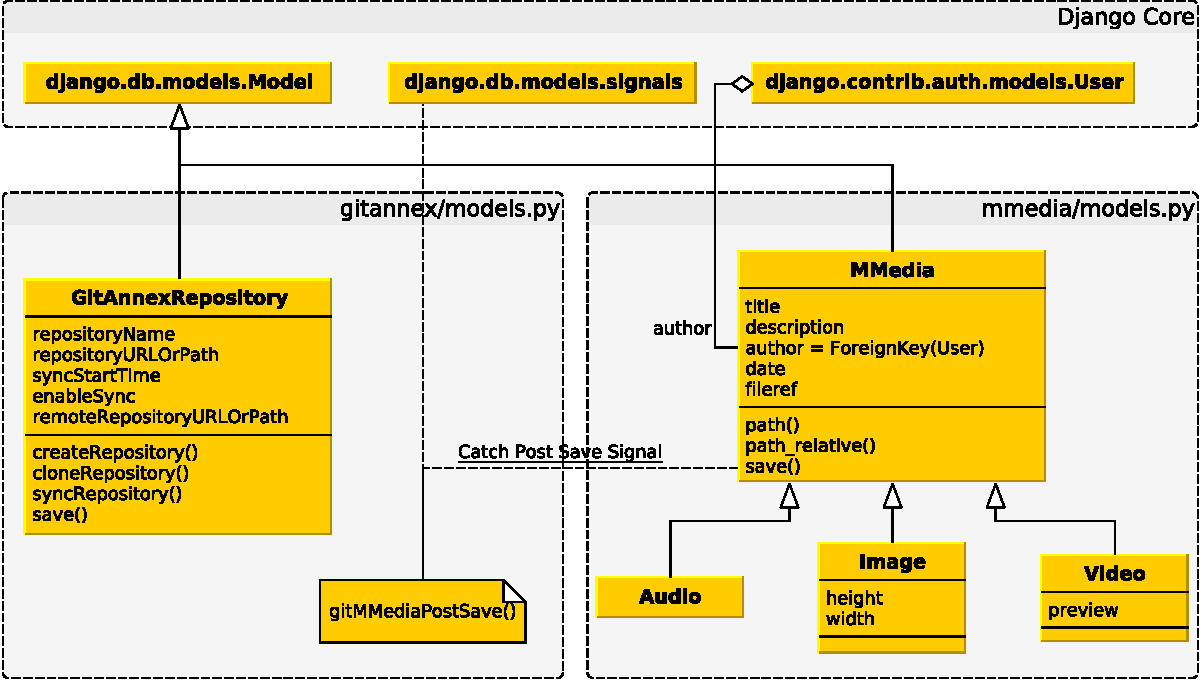
\includegraphics[width=\textwidth]{./Figure/UML_Schema_Django-crop.pdf}
  \rule{35em}{0.5pt}
  \caption[Esquema UML das aplicações Django]{Esquema UML das aplicações Django.}
  \label{fig:SchemaUMLDjango}
\end{figure}

\subsection{Mocambos\_Portal\_Local}
\framebox[\textwidth]{\footnotesize O código esta disponível no
  \url{https://github.com/RedeMocambos/Mocambos_Portal_Local}}

O \emph{script bash}, \verb|script/install-django-env.sh|, instala os
pacotes de sistema necessários, e também cria o ambiente virtual,
usando o programa \emph{virtualenv}\footnote{\emph{Virtualenv} è um
  Software Livre para criar ambientes Python isolados disponível no
  \url{http://www.virtualenv.org}.}, que permite instalar facilmente
versões específicas de bibliotecas e do interprete Pyhton, além do
Django, sem alterar as versões já instaladas no sistema. Na pasta
\verb|exemplos/| se encontram alguns arquivos de configuração de
exemplo, pré-configurados para a conexão ao servidor LDAP da RM (ver
\ref{MocambosLDAP}).


\subsection{Django mmedia}
\framebox[\textwidth]{\footnotesize O código esta disponível no
  \url{https://github.com/RedeMocambos/mmedia}}

A aplicação \emph{mmedia} implementa o modelo de dados multimídia com
suporte par o armazenamento em repositório \emph{git-annex}.

Os modelos, em \emph{Django}, precisam ser criados no arquivo \verb|model.py|,
onde, primeiramente, definimos a estrutura de base da classe
\emph{MMedia}, com os atributos comuns para todos os objetos
multimídia. As classes \emph{Audio}, \emph{Image} e \emph{Video},
herdam os atributos da classe abstrata ``MMedia'', acrescentando outros
atributos específicos para o tipo de objeto.

Os objetos são salvos no \emph{database}, e serializados no disco
através o \emph{overriding} da função \emph{save()}:

\begin{code}
    def save(self, *args, **kwargs):
        logger.debug(type(self))
        serializeTo = os.path.join(settings.MEDIA_ROOT,\
                                   settings.GITANNEX_DIR,\
                                   settings.PORTAL_NAME,\
                                   settings.SERIALIZED_DIR,\
                                   os.path.basename(self.fileref.path)+ '.xml')
        logger.info('>>>> Serialize to: ' + serializeTo)
        out = open(serializeTo, "w")
        XMLSerializer = serializers.get_serializer("xml")
        xml_serializer = XMLSerializer()
        xml_serializer.serialize((self, ), stream=out)
        super(MMedia, self).save(*args, **kwargs)
\end{code}


\subsection{Django gitannex}
\framebox[\textwidth]{\footnotesize O código esta disponível no
  \url{https://github.com/RedeMocambos/gitannex}}

A aplicação \emph{gitannex} implementa parte do modelo de dados de um
repositório \emph{git-annex} no \emph{Django}, acrescentando os
atributos e as funcionalidades necessárias para a planejamento da
sincronização.

\begin{figure}[htbp]
  \centering
  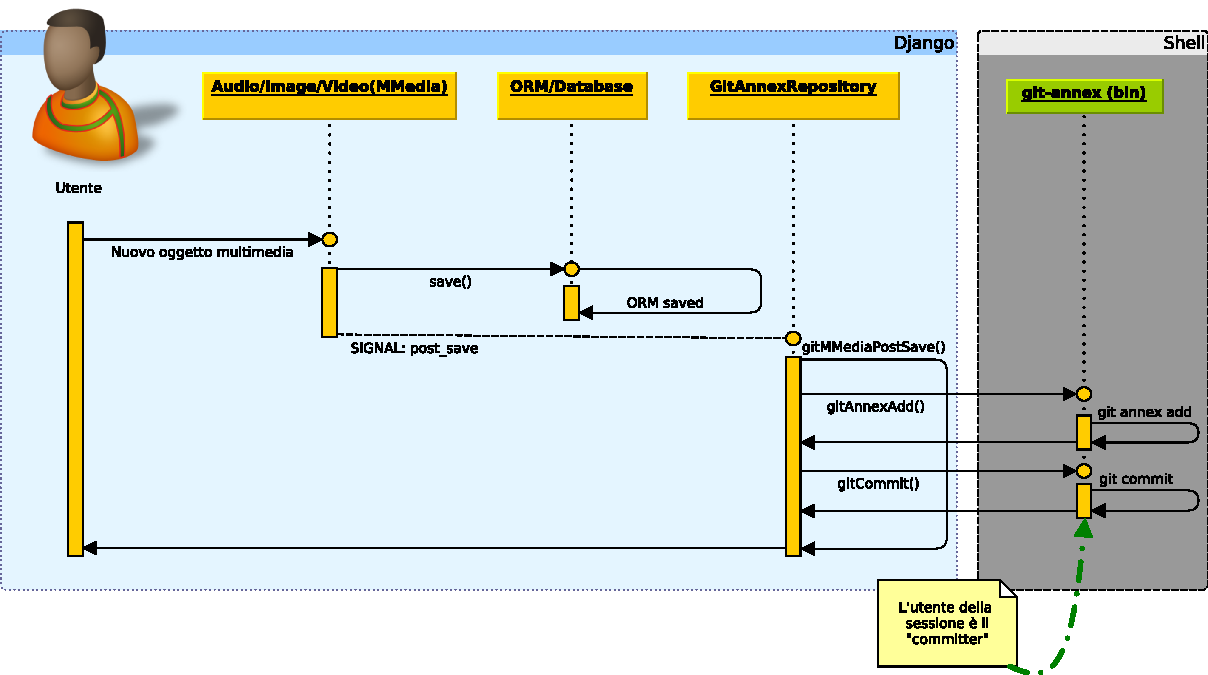
\includegraphics[width=\textwidth]{./Figure/SequenceDiagram_NuovoOggetto-crop.pdf}
  \rule{35em}{0.5pt}
  \caption[Diagrama de sequencia da criação de um novo objeto
  multimídia]{Diagrama de sequencia da criação de um novo objeto
    multimídia.}
  \label{fig:SequenceDiagramAdd}
\end{figure}

Seguindo a especificação, é definido, através do atributo
\emph{syncStartTime}, um horário para o inicio da sincronização, que é
inicializada pela função \emph{runScheduledJobs()}. Para interagir
mais facilmente com o framework através do terminal é possível definir
comandos que precisam ser criados na pasta
\verb|management/commands/|, onde se encontra, por exemplo, o comando
\verb|run_scheduled_jobs| que chama a função homônima. Desta maneira
é possível executar operações planejando-as através do
\emph{cron}\footnote{``Em sistemas operacionais Unix e Unix-like, o
  comando crontab permite o planejamento de comandos, ou seja permite
  de agendá-los no sistema para serem executados periodicamente.'',
  traduzido de Wikipedia:
  \url{http://it.wikipedia.org/wiki/Crontab}.} o diretamente no
terminal com:
\begin{verbatim}
zumbi@palmares:~$ python manage.py run_scheduled_jobs
\end{verbatim}

\emph{Django} providencia um sistema de sinais, enviados em
concomitância de operações como a \emph{save()} de um objeto, que
podem ser interceptados em outras partes do sistema. A aplicação
\emph{gitannex} intercepta o sinal padrão do Django, \emph{post-save}
(ver figura \ref{fig:SequenceDiagramAdd}), em objetos que herdam da
classe \emph{MMedia}\footnote{Django não suporta a ``filtragem'' de
  sinais enviados por subclasses de uma classe dada, neste caso
  \emph{MMedia}. Para isso, foi usado um truque encontrado na rede
  (ver o código no arquivo \texttt{gitannex/signals.py}).}, através da
função \emph{gitMMediaPostSave()}:

\begin{code}
@receiver_subclasses(post_save, MMedia, ``mmedia_post_save'')
def gitMMediaPostSave(instance, **kwargs):
    logger.debug(instance.mediatype)
    logger.debug(type(instance))
    logger.debug(instance.path_relative())

    path = instance.path_relative().split(os.sep)
    if gitannex_dir in path:
        repositoryName = path[path.index(gitannex_dir) + 1]
        gitAnnexRep = GitAnnexRepository.objects.get(\
                      repositoryName__iexact=repositoryName)
        gitAnnexAdd(os.path.basename(instance.fileref.name),\
                    os.path.dirname(instance.fileref.path))
        gitCommit(instance.title, instance.author.username,\
                  instance.author.email, os.path.dirname(instance.fileref.path))
\end{code}
